\documentclass[phd,tocprelim]{cornell}
\let\ifpdf\relax

\usepackage{amsmath}
\usepackage{amsthm}

%%%%%%%%%%%%%%%%%%%%%%%%%%%%%%%%%%%%%%%%
                                       %
% change this line for portable code:  %
\newcommand*{\commonDir}{../common/}   %
\input{\commonDir preambleCommon}      %
                                       %
%%%%%%%%%%%%%%%%%%%%%%%%%%%%%%%%%%%%%%%%


\graphicspath{{./figures/}{../falconBioinfo/figures/}%
{../epistasisSameGeneArXiv/figures/}}

% Document specific
% (it is empty)
%%%%%%%%%%%%%%%%%%%



%
% tocprelim option must be included to put the roman numeral pages in the
% table of contents
%
% The cornellheadings option will make headings completely consistent with
% guidelines.
%
% This sample document was originally provided by Blake Jacquot, and
% fixed up by Andrew Myers.
%
% ************* TODO (Brandon Barker) ***********************************
%
%General
% TODO (Brandon Barker)
% Read Formatting Rules on Grad School site.
%  - referencing figures/capitalization: \Fig~or fig or figure ...
%
% Spellcheck
%
% Permissions: Once title of thesis is known, write permission letter to use publications
% http://www.proquest.com/assets/downloads/products/UMI_CopyrightGuide.pdf
% E-mail Wiley @ permissionsus@wiley.com
%
%
% Word histogram to check for words used too often.
%

% Chapter 1: Introduction:
% Add other (Jason-deleted) sections/words - update correct figure 1
% Figure 2: self-reference full article when mentioned.
% Reference arXiv preprint along side Lee2012
% Epistasis
%
% Chapter 2: Using FBA to understand epistasis dynamics.
%
% -- Add short appendix on the software.
%
% Interlude: discuss limitations of FBA for epistasis, etc (e.g. Papp, beneficial mutations).
%
% Chapter 3: FALCON
% 
% Chapter 4: MILP-FALCON/whole-cell-model
%
% Chapter 5: An improved undestanding of epistasis
%

% Consider adding the Motif/model work somehow?


%Chapter 3:
%
% Figure/table: be sure to show the differences for minDisj and
% original method on the human network, somehow.
%
% Do I discuss the issue of negative fluxes in the FALCON objective?
%
% Parameter sensitivity analysis for initial flux
% scaling value.
%
% Consider discussing ass:chap and ass:rate in the text.
% Perhaps discuss related to ass:rate that a penalty deriving
% from mass-action considerations is warranted - cite Karr2012
%
% Relatedly, discuss how how min(a,b) is a good approximation
% to mass-action assumptions -- need to think about this:
% since mass action would propose r = [a][b], then we would have
% log(r) = log(a) + log(b) ... hmm
%
%
% Discuss Assumption: complexation formation assumption (recall Tom Fox's talk)
% Discuss Assumption: Localization (Pablo Meyer, IBM):
%     http://researcher.watson.ibm.com/researcher/view.php?person=us-pmeyerr
% 
%
% Add discussion on atomic (Lee et al) versus batch direction
% assignment.
%
% Fix missing references.
%
% Tie in motivating rules example with previous section
% showing the merits of CNF
%
% Add another illustrative figure.
%
% Add a table/figure comparing estimated EC abundance using
% e.g. original method vs our method, also for fluxes.
% - Benchmark these against cancer data in Chapter 5
%
% Discuss incrementing flux_sum at each iteration.
%
% Figure out how copyright registration is handled; apparently it is necesasry.
% I assume it is handled by Cornell.
%

% ************* End of TODO ***********************************************
%Added by Brandon:
%\usepackage[amsmath,amsthm,thmmarks]{ntheorem}
\usepackage{hyperref}


%if you're having problems with overfull boxes, you may need to increase
%the tolerance to 9999
\tolerance=9999

%\renewcommand{\caption}[1]{\singlespacing\hangcaption{#1}\normalspacing}
\captionsetup{compatibility=false}
\renewcommand{\caption}[1]{\singlespacing\caption{#1}\normalspacing}

%
%\bibliographystyle{plain}
%\newcommand{\citep}[1]{\cite{#1}}
%\newcommand{\citealt}[1]{\cite{#1}}
\usepackage[numbers,sort&compress]{natbib}
\bibliographystyle{unsrtnat}
\setlength{\bibsep}{24pt}
%

\title {Advances in Genome-Scale Modeling Applied to Expression-based
Flux Estimation and Epistasis Prediction}
\author {Brandon Barker}

\conferraldate {August}{2014}
\degreefield {Ph.D.}
\copyrightholder{Brandon Elam Barker}
\copyrightyear{2013}


%%%%%%%%%%%%%%%%%%
\begin{document}%%
%%%%%%%%%%%%%%%%%%

\newboolean{thesisStyle}
\setboolean{thesisStyle}{true}

%%%%%%%%%%%%%%%%%%%%%%%%%%%%%%%%%%%%%%%%
                                       %
\input{\commonDir documentHeadCommon}  %
                                       %
%%%%%%%%%%%%%%%%%%%%%%%%%%%%%%%%%%%%%%%%

\maketitle
\makecopyright

\begin{abstract}

Quantitative models are increasingly being used to interrogate the
metabolic pathways that are contained within complex biological
processes, and at a higher level, these models are used to explore
questions in population genetics with complex physiological processes
absent in typical, idealized population genetic models.  I give an
overview of constraint-based modeling and its purview in the field of
metabolic modeling. By using a simple version of constraint-based
modeling known as flux balance analysis, we elucidate patterns that
occur in gene-gene interactions of deleterious mutations and the
influences that metabolic network architecture may bring to bear on
adaptation. We then turn to developing approaches that enable the
simulation of beneficial mutations, allowing the study of effects of
different parameters on genetic interaction patterns occurring during
environmental adaptation. Because many of these approaches rely on
establishing a physiologically accurate flux for the wild-type
organism, we address the problem of estimating metabolic fluxes using
gene expression data and constraint-based models. Finally, this
methodology is employed in the separate context of cancer metabolism
analysis.
\end{abstract}

\begin{biosketch}
Your biosketch goes here. Make sure it sits inside
the brackets.
\end{biosketch}

\begin{dedication}
\begin{center}
\textit{To my parents---James and Carol Barker, \\
For their love, time, and beneficence, \\
Without which this work would not have been possible. \\
\vspace{10 mm} 
To my wife, Lin Xue, \\
For giving me the momentum to pursue graduate school, \\
For her patience while I studied, \\
For her continuing love and , \\
And most importantly, for being an amazing mother.\\
\vspace{10 mm} 
To my son, Lindon Barker, \\
For your extra motivation towards finishing in a timely manner, \\
And for your terrific smiles, grins, and laughs during this last year.}
\end{center}
\end{dedication}

\begin{acknowledgements}
Firstly I would like to thank my advisor,  Zhenglong Gu, under
whose supervision this work has unfolded, and who has provided me with
substantial support, encouragement, and irreplaceable mentoring. I owe
much to my colleague and friend, Lin Xu, for not only showing me
the ropes and giving me hope, but also getting me interested in so
many topics in evolution; much of the present work, particularly that
involving epistasis, would not have happened without him. Without
Jason Locasale's intellectual incitation and advice, I never would
have wandered down the path to what has, to me, become the most
interesting part of this work, nor the path to the Big Red Barn quite
so much as I did. My thesis committee members---David Christini,
Chris Myers, and Michael Stillman---have provided much advice
over the years, scientific and otherwise.

My other collaborators in the present work include Tim Connallon,
whose knowledge on epistasis surpasses anyone I know, and similarly
for Alex Shestov with regard to metabolic flux analysis;
Kieran Smallbone, who has given helpful advice over the years 
regarding constraint-based models, as well as having helped develop several  
algorithms and models that I have employed in this work, including one in 
particular that served as the impetus for some of the research in the latter 
chapters; Yiping Wang, a phenomenal young researcher who helped
with some analysis in the last chapter during his first month on
campus, and Hongwei Xi, for providing substantial support for his
programming language ATS, which was employed in the latter chapters.

In the lab, Xiaoxian Guo, Huifeng Jiang, and Zhe Wang
provided much experimental advice, training, and data.

I would also like to thank many other colleagues for their help,
friendship, scientific discussion, or some combination of
the three. These include Diana Chang, Elijah Bogart, 
Hong Chian, Martha Field, Lei Huang,
Haley Hunter-Zinck, Ben Heavner, Xiaojing Liu, Henry Lu, Anuttama Mohan,
Lonnie Princehouse, Narayanan Sadagopan, and Kaixiong Ye.

Without the stimulus, confidence, and aid from my early mentors at the
University of Kentucky, this document would not exist; in particular,
I thank Ruriko Yoshida, for renewing my passion in science,
Jim Lund, for being my first biology mentor (and providing the
opportunity to become acquainted with my wife), Jerzy Jaromczyk
for his friendly help and advice throughout and beyond my
undergraduate education, and to Henry Dietz, for being a great
educator and advising my senior design project.  My passionate and
reassuring high school biology teacher, David Christiansen,
warrants special thanks for being continually amazed at the wonders
biology has to offer. Lastly, I thank my friend Benjamin Runyon,
for always lending an ear.
\end{acknowledgements}

\contentspage
\tablelistpage
\figurelistpage

\normalspacing \setcounter{page}{1} \pagenumbering{arabic}
\pagestyle{cornell} \addtolength{\parskip}{0.5\baselineskip}

\chapter{Introduction}

There has been a surge of interest in understanding the regulation of
metabolic networks involved in disease in recent years.  Quantitative
models are increasingly being used to interrogate the metabolic
pathways that are contained within this complex disease biology.  At
the core of this effort is the mathematical modeling of central carbon
metabolism involving glycolysis and the citric acid cycle (referred to
as energy metabolism).  Here we discuss several approaches used to
quantitatively model metabolic pathways relating to energy metabolism
and discuss their formalisms, successes, and limitations.  Your
abstract goes here. Make sure it sits inside the brackets. If not,
your biosketch page may not be roman numeral iii, as required by the
graduate school\introSameGeneCredit.

The accumulated amount of biochemical work carried out over the years
has elaborated complex metabolic systems and networks.  This
information includes the network architecture encoded in chemical
reactions that are carried out by metabolic enzymes and the kinetic
parameters that determine reaction mechanisms involved in each of
these chemical reactions.  Application of this knowledge has led to
tremendous predictive capability in characterizing metabolic
regulation in normal physiology including the growth of unicellular
organisms and the successful simulation of energy metabolism in
healthy red blood cells.  However, there are far fewer instances in
which these models have been applied to the characterization of
pathophysiology.  Applying our knowledge of metabolic regulation to
the investigation of disease states such as cancer or
neurodegeneration is currently a scientific frontier.  In this review,
we will revisit several classic techniques for the mathematical
modeling of metabolic pathways and discuss instances where their
application to biomedical science is beginning to yield fruitful
dividends.

\section{Linear Systems, Flux Balance Analysis}
Linear models are mathematical models that contain a set of algebraic
equations based on the stoichiometric relationships that define
conservation relationships within a metabolic network.  Linear models,
to our knowledge, were first applied to biochemical systems in 1961 by
Howard Shapiro \citep{Shapiro1961}. Shapiro discussed the possibility
of using optimization in biochemical linear models in a 1969
publication \citep{Shapiro1969}. In 1984, a model incorporating
glycolysis and the TCA cycle was employed running a variant of
Dantzig’s algorithm with the assumed biological objective of minimized
free energy dissipation \citep{Panne1985, Watson1984}. An enduring
research program was initiated by Bernhard Palsson half a decade later
\citep{Savinell1992a, Savinell1992}. One of Palsson's early works
showed that growth maximization in an \textit{E. coli} model could
correctly match 86\% of 79 gene essentialities examined
\citep{Edwards2000}. Subsequent modeling in \textit{S. cerevisiae} was
able to closely predict growth rates and exometabolic fluxes in
various media, and nearly capture the in vivo phosphate/oxygen (P/O)
ratio of 0.95 with a simulated P/O value of 1.04, showing that models
of eukaryotes were also feasible \citep{Famili2003}. If one chooses
the biological objective function to reflect the appropriate
physiological demands then it is possible to predict features of
adaptation; this was shown to be the case for growth optimization in
several E. coli mutants \citep{Fong2004_sb2013}. By this time it had
become apparent that linear models held much promise, particularly
when coupled with optimization.


\section{Genome Scale Modeling}
Today, when we refer to linear models, we most often mean Constraint
Based Models (CBMs). We refer to a CBM as any model making use of the
stoichiometric matrix, $\mathbf{S}$, as a linear matrix constraint, e.g. $\mathbf{SF} =
\mathbf{0}$, where $\mathbf{F}$ is a flux vector\footnote{$F$ is usually used to denote a
steady state flux, whereas $v$ is used for fluxes more generally. In
much of the genome-scale constraint-based modeling literature, $v$ is
used in all cases}. In fact, this is a nearly universal
constraint, as it guarantees conservation of mass during steady state
processes such as exponential growth or tissue maintenance \citep{Fleming2012}. 
Other constraints commonly used include reversibility constraints when the
direction of a reaction is known for physiological conditions of
interest, bounds on the uptake of nutrients or efflux rates due to
regulation or physiology, or bounds on enzyme reactions when the
maximum enzyme velocity $V_{max}$ is known.

\begin{figure}
\centering
  \includegraphics[width=0.75\textwidth]{SmatExample}
\caption{A simple geometric illustration of an FBA problem
\textbf{(a)}. Constant constraints on the $F_i$ limit the feasible
solution to an n-dimensional cube (shown in grey). Further linear
constraints from the $\mathbf{S}$ matrix create a cone of feasible solutions
(blue). Linear programming algorithms find an optimal solution on a
vertex (illustrated with orange circle). Depiction of a simple
metabolic network with compartmentalization and its associated
stoichiometric matrix \textbf{(b, c)}. The three compartments denoted
with subscripts $b$, $e$ and $c$ represent the boundary, extracellular
environment, and cytosol, respectively. The boundary is what separates
the model from its environment, and mass balance is not assumed at the
boundary; this allows for the implementation of source and sink
reactions.}
\label{fig:SmatExample}
\end{figure}


Because these constraints give rise to an underdetermined system, it
will not be possible to identify a unique solution for the flux
vector. A unique solution is often desirable as it allows
investigators to analyze a putative metabolic phenotype. Indeed, this
is one of the more convenient features of linear optimization: the
ability to get meaningful solutions without explicitly taking into
account any, or at least very few, free parameters.  Flux Balance
Analysis, or FBA, assumes a linear combination of fluxes to be
maximized or minimized (\Fig~\ref{fig:SmatExample}). In microbes, perhaps the most popular
FBA objective has been growth maximization, which consists of the
biomass precursors and products formulated as a single
pseudo-reaction. Additionally, an ATP maintenance constraint should be
formulated as a sink reaction with the molar ATP required to keep one
gram of dry weight biomass living for one hour \citep{Varma1994}. This empirically
determined constraint, although assumed, is less discussed, perhaps
due to its dependence on individual strains and environments.  We note
that for many expression-based methods in the CBM framework, the ATP
maintenance constraint is not required (see Table~\ref{tab:CBMmethods}
and \Fig~\ref{fig:FluxomicsTools} for
examples). Fixed biomass objectives by themselves also have some
undesirable qualities; biomass composition likely has some measure of
variability based on genetic background and environment.  Robust FBA
attempts to address this problem by allowing some variation in the
biomass composition, as determined by variation of empirical assays of
biomass \citep{Zavlanos2011}. Despite these caveats, FBA has recently been found to not
only predict growth in microbes, but also has good agreement with gold
standard 13C flux assays in vivo when the growth objective is used
along with ATP synthesis maximization and minimization of absolute
fluxes \citep{Schuetz2012}.

\newcolumntype{L}[1]{>{\raggedright\let\newline\\\arraybackslash\hspace{0pt}}m{#1}}
\begin{table*}
\centering
%\resizebox*{\textwidth}{\textheight}{\begin{minipage}{\textwidth}%
\newlength\textnofoot
\setlength{\textnofoot}{\textheight-\footskip}
\resizebox*{\textwidth}{\textnofoot}{%
\begin{tabular}{|L{3cm}|L{4cm}|L{4cm}|L{4cm}|L{4cm}|L{4cm}|}
\hline
\textbf{Method Family} & \textbf{Description} & \textbf{Benefits} &
\textbf{Caveats} & \textbf{Solver Type} & \textbf{Notes}
\\ \hline
FBA \citep{Orth2010} & Flux Balance Analysis: Linear programming
applied to the model. & Usually very fast and simple to use,
especially when a biomass pseudo-objective is available. & Arguably
has more limited use in non-microbial models. Only simple objectives
or sequential (e.g. bi-level) optimization is practical. & Linear &
Often constraint-based modeling (CBM) in general may be referred to as
FBA, though this is not technically correct.
\\ \hline
MoMA \citep{Segre2002_sb2013, Shlomi2005} & Minimization of Metabolic
Adjustment & Usually very fast and simple to use, especially when a
reference or wild-type flux is available; useful for simulating
mutations. & It has been argued that the closest distance to a flux
doesn't represent mutation as well as simulating the least number of
flux changes (ROOM). & Linear, Quadratic Convex & Related, but
slightly more sophisticated methods are being used to estimate flux
profiles from expression data.
\\ \hline
DFBA \citep{Varma1994} & Dynamic FBA: incorporates a step-wise
simulation of FBA, along with update rules that relate biomass to
uptake rate, solving for extracellular concentrations. & Allows for
some non-steady state observations & Small timescale dynamics and
intracellular dynamics may be difficult to model. & Linear (Iterative)
& Other, but infrequently used (due to difficulty) methods involving
regulation (rFBA) or multi-scale models of tissues build on this
approach.
\\ \hline
EBA \citep{Fleming2012, Schellenberger2011, Beard2002, Henry2007} &
Energy Balance Analysis: FBA, but also incorporates thermodynamic
constraints & Incorporates thermodynamic information, prevents futile
cycles. & Usually much slower than LP methods like FBA. & nonlinear,
MILP, or Monotropic & A highly active research area.
\\ \hline
Tissue-specific Model Creation \citep{Wang2012, Becker2008,
Shlomi2008} & Requires expression data for tissue of interest. &
Tissues have vastly different regulatory schemes; these methods take
this into account by finding which metabolic genes are likely to be
expressed in a given tissue. & Still requires some other method and
objective to estimate flux or do pathway analysis. & MILP & A highly
active research area.
\\ \hline
Expression-Flux mapping \citep{Lee2012, Chandrasekaran2010a} & Takes
ideas from MOMA and tissue-specific model creation to estimate
fluxes. & Unlike tissue-specific models, will actually estimate the
flux since a MOMA-like objective is employed. & Requires high-quality
(e.g. RNA-Seq) expression data, or for PROM, abundant microarray data
from different conditions. & Linear optimization, but moderate number
of simulations or preprocessing required. & Highly accurate
predictions can be obtained.
\\ \hline
Interaction Search \citep{Imielinski2010, Imielinski2008, He2010,
Xu2012} & Epistasis, or genetic interactions, come up in many
contexts, but are also important in energy metabolism, since energy is
often related to very important phenotypes including growth,
proliferation, and survival. & For such analyses, convex optimization
may offer the only tractable method. & Simulating pairwise epistasis
in the general case requires pairwise simulation of all double mutants
of interest, which can be very time-consuming at the genome scale when
different mutations in each gene, or different environments, are
considered & Linear optimization, but often many simulations
required. Min Cuts (exponential). & The sign of weak epistasis is
difficult to predict, due to error propagation in growth rates.
\\ \hline
\end{tabular}}
\caption{ Families of methods for constraint-based models. Broad
classes of methods are described, along with references to some
individual implementations or studies.}
\label{tab:CBMmethods}
\end{table*}


\begin{figure}
\centering
  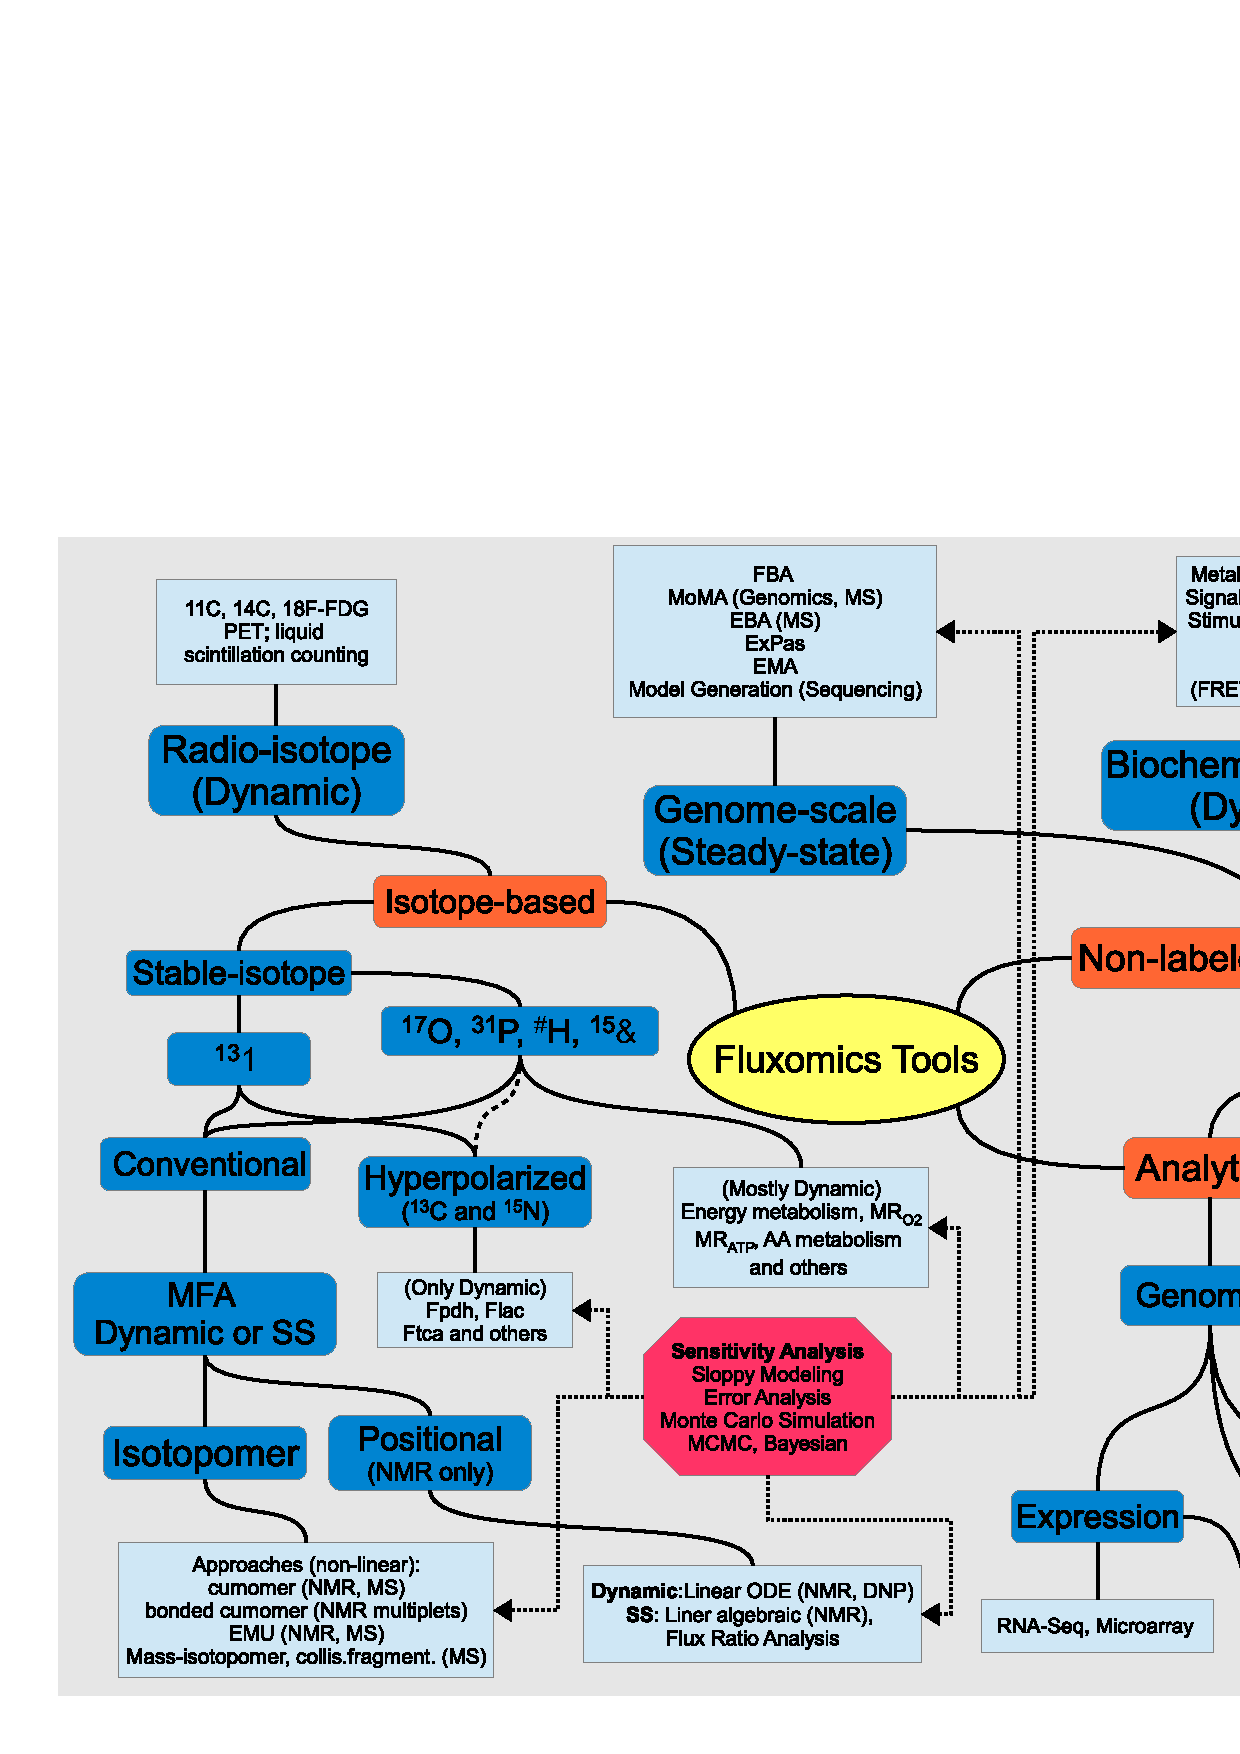
\includegraphics[width=\textwidth]{FluxomicsTools}
\caption{Schematic representation of fluxomics tools. Important to
fluxomics are both the mathematical and computational tools for
nonlabeled and labeled techniques, as well as the analytical methods
used to obtain data and parameters. In the current work we focus only
on nonlabeled genome-scale steady state and related analytical
methods, but a full description can be found
\protect\citep{Shestov2013a}. Sequence data is employed in the
construction of organism models, whereas proteomics and expression
data find use in the creation of tissue or cell-type-specific
models. High-quality expression data such as RNA-seq and ribosomal
footprinting are beginning to find uses in flux prediction. Several
prominent genome-scale techniques include flux balance analysis (FBA),
minimization of metabolic adjustment (MoMA), energy balance analysis
(EBA), ExPas (extreme pathways), and elementary mode analysis
(EMA). Nonlabeled techniques along with genome-scale analysis include
biochemical kinetics modeling tools to study metabolic and signaling
networks and their regulation architecture with established tools like
metabolic control analysis (MCA) and global sensitivity analysis
(GSA). Additional sensitivity analysis should be conducted, e.g., with
Monte-Carlo techniques like Markov chain Monte-Carlo (MCMC, Bayesian)
analysis to check the reliability of extracted metabolic parameters,
including fluxes.}
\label{fig:FluxomicsTools}
\end{figure}


Minimization of absolute flux is a commonly used objective employed
alongside other objectives, forming a minimax problem (i.e. finding
the minimum absolute flux profile among all flux profiles that
maximize biomass). This approximates the biological goal of being
efficient with enzyme production costs and enzyme crowding constraints
while also guaranteeing that no thermodynamically impossible loops are
present, that is, ruling out some fluxes that might otherwise violate
Kirchoff’s loop rule \citep{Smallbone2009a, Schellenberger2011}.  This
constraint will work whenever a sink reaction, such as growth, is
being optimized.  However, maximizing an internal flux, as in Flux
Variability Analysis \citep{Orth2010}, could still result in internal
cycles \citep{Schellenberger2011}. Initial thermodynamic approaches
involved nonlinear optimization \citep{Beard2002, Henry2006,
Henry2007, Kummel2006}. Constraints satisfying Kirchoff’s loop rule
were later developed that were faster and more generally applicable
than prior methods \citep{Schellenberger2011, Muller2013}.  Still,
these involve integer constraints that put this problem in a slower
class of algorithms than the convex minimized absolute flux problem.
When available, thermodynamic data is valuable; it can not only be
used to guarantee there are no internal cycles, but can also aid in
determining reaction direction and potential regulatory targets
\citep{Schellenberger2011, Henry2006, Haraldsdottir2012,
DeMartino2012}. Application of this framework to concentration data
allows unmeasured metabolite concentrations to be inferred and global
concentrations to be resolved at the organelle level
\citep{Kummel2006}. CBMs have also found use in tracing individual
atoms through pathways, which provides a more appealing framework for
performing Metabolic Flux Analysis (MFA; discussed below) on stable
isotope data due to the lack of bias compared to typical MFA models,
which are often an order of magnitude smaller than genome-scale
reconstructions \citep{Ravikirthi2011}.  Recent insightful work has
made it possible to simplify the computational complexity of loopless
FBA to be nearly the same as conventional FBA, but some mathematical
difficulties must still be overcome before bounds on exchange fluxes
can be suitably incorporated for genome-scale modeling
\citep{Fleming2012, Warren2007}.


The metabolism of different tissues within the same organism is
diverse; whereas the metabolism in liver is anabolic, neurons or red
blood cells have a much more limited catabolic regime
\citep{Lewis2010, Jamshidi2006, Wang2012}.The creation of tissue
specific models for multicellular organism has become an important
problem, and several automated algorithms taking as inputs tissue
expression data and a generic model for the organism have been
developed \citep{Wang2012, Becker2008, Shlomi2008}. Coupling multiple
cellular models together will enable multi-scale modeling of tissues
in multicellular models or entire ecosystems for microbes
\citep{Lewis2010, Sun2012, Bordbar2010, Klitgord2011}.

Automated generation of metabolic networks from genome sequence and
pathway databases, especially in prokaryotes, has been developed
\citep{Seaver2012, Aziz2012, Henry2011, Faria2013}.  This will offer
many advantages to modelers: a starting point for curated models (a
draft reconstruction is estimated to often take several months even in
prokaryotes), a means for doing population or ecological simulation
\citep{Klitgord2011}, and personalized genomic modeling for patients
with metabolic syndromes such as cancer where both the patient and
possibly the disease have diverse genotypes \citep{Locasale2012,
Folger2011}.  Eukaryotic models are somewhat more difficult to
generate due to the necessity of protein localization and metabolite
transporter information \citep{Seaver2012}. Automatic reconstruction
going beyond enzymatic gene information, such as rFBA models, should
also be possible \citep{Covert2001, Herrgard2006c}; the automated
generation of Boolean and higher-order discrete regulatory models
using time-series expression data has been explored as well, though to
date these regulatory models have not been coupled to metabolic
reconstructions \citep{Dingel2009, Dimitrova2009, Stigler2007a,
Jarrah2007}. These approaches and other families of genome-scale
methods are discussed in Table~\ref{tab:CBMmethods}.

Several approaches have been used in applying CBMs to cancer and the
Warburg effect, the preference for glycolytic ATP production over
glucose-derived mitochondrial ATP production in cancer cells 
\citep{Resendis-Antonio2010a, Shlomi2011, Vazquez2011}. An
important study working with a simplified, small model of
central-carbon metabolism showed that, while the TCA cycle predicts
better ATP yield than glycolysis when only available glucose is
considered as a constraint, the addition of enzyme solvent-capacity
constraints creates a preference for ATP synthesis through
glycolysis \citep{Vazquez2011}. More recently, the work of Vazquez et al. was extended
to include a genome-scale model along with enzyme solvent-capacity
constraints, which was able to show significant correlations between
fluxes and expression in the NCI-60 cell line panel, as well as
predicting an intermediate state in cancer metabolism transition
exhibiting a temporary increase in OxPhos that was supported by two
prior experimental observations \citep{Shlomi2011}. All of these
approaches correctly predicted lactate production. Concurrent research
on predicting cancer targets by screening for simulated negative
epistasis in cancer tissue-specific models that have at least one
known-drug target and no known effect on normal tissue revealed many
epistatic interactions \citep{Folger2011}. A related study confirmed
one of these synthetic lethalities between hemeoxygenase and fumarate
hydratase, a mutation found in certain kidney cancers
\citep{Frezza2011}. The recent publication of Human Recon~2 promises
to aid in the understanding of many human diseases; already 65
cell-type specific models based on it are available, and the model
reports 77\% accuracy in identifying metabolic markers across 49
inborn errors of metabolism \citep{Thiele2013}. Although this model is
a great step forward in consolidating much of the knowledge about human
metabolism, it is only one of many steps to come. For instance, this
model is still primarily only amenable to steady-state approaches,
lacks corresponding enzyme-regulatory and signaling architecture, and
has introduced more dead-end metabolites than it removed (1,176 versus
339). 

\section{Conclusions for the State of Linear and Genome-Scale Models}
Kinetic models for smaller pathways are possible when the data are
present, but many energetic questions concern the entire cell, leaving
only incorporation of CBMs as a viable option. The original efficiency
and ease of use of FBA have helped propagate a field of more diverse
algorithms that are often tractable on today’s computers using the
same modeling and software frameworks \citep{Gianchandani2009,
Lewis2012_sb2013}.  Numerous methods and successful applications in
energy metabolism exist, including prevalent diseases such as heart
disease, cancer, and Alzheimer’s \citep{Sangar2012}.

Multiscale models, as were used in the Alzheimer’s models, will
undoubtedly become more common. At the intracellular scale, CBMs are
also beginning to incorporate information other than metabolic
stoichiometry \citep{Lerman2012, Karr2012, Yizhak2010}. 
A whole cell model for \textit{Mycoplasma genitalium}
incorporating information about all classes of macromolecular
synthesis and degradation, in addition to stoichiometric and
regulatory information, found a non-stochastic coupling between
metabolism and the cell-cycle where DNA replication rates depended on
the concentration of dNTP \citep{Karr2012}. Models like these are not easy to build,
but substantial endeavors are underway to assist in their draft
construction and refinement, and together with an increase in use of
jamboree meetings of organism and model experts and online
collaborative tools, will likely aid in creating public models of
higher quality and the understanding of many biological processes
outside the traditional scope of metabolism \citep{Aziz2012,
Thiele2013, Herrgard2008, Karr2013, kbase2013, Pabinger2011,
Helikar2012}.


%\begin{equation}
%k_1=\frac{\omega }{c({1/\varepsilon_m + 1/\varepsilon_i})^{1/2}}=k_2=\frac{\omega
%sin(\theta)\varepsilon_{air}^{1/2}}{c}
%\end{equation}
%
%\noindent
%where $\omega$ is the frequency of the plasmon, $c$ is the speed of
%light, $\varepsilon_m$ is the dielectric constant of the metal,
%$\varepsilon_i$ is the dielectric constant of neighboring insulator,
%and $\varepsilon_{air}$ is the dielectric constant of air.

\chapter{Dynamic Epistasis for Different Alleles of the Same Gene}

\section{Introduction}
\epiSameGeneAbstract

%%%%%%%%%%%%%%%%%%%%%%%%%%%%%%%%%%%%%%%
%                                     %
\input{\commonDir epistasisSameGene}  %
%                                     %
%%%%%%%%%%%%%%%%%%%%%%%%%%%%%%%%%%%%%%%

\chapter{Dynamic Epistasis Under Varying Environmental Perturbations}

\hl{it is empty}


\chapter{A robust and efficient method for
estimating enzyme complex abundance
and metabolic flux from expression data}

\falconAbstractMotivation \falconAbstractResults

%%%%%%%%%%%%%%%%%%%%%%%%%%%%
%                          %
\input{\commonDir falcon}  %
%                          %
%%%%%%%%%%%%%%%%%%%%%%%%%%%%


\chapter{Epistatic Landscapes Arising from Adaptive Mutations}
\epiBeneMutAbstract
%%%%%%%%%%%%%%%%%%%%%%%%%%%%%%%%%%%%%%%%%%%%%%%
%                                             %
\input{\commonDir epistasisBeneficialMutant}  %
%                                             %
%%%%%%%%%%%%%%%%%%%%%%%%%%%%%%%%%%%%%%%%%%%%%%%


\appendix

\chapter{Supporting Information for
Dynamic Epistasis for Different Alleles of the Same Gene}

%%%%%%%%%%%%%%%%%%%%%%%%%%%%%%%%%%%%%%%%%%%%%%%%
%                                              %
\input{\commonDir epistasisSameGene_appendix}  %
%                                              %
%%%%%%%%%%%%%%%%%%%%%%%%%%%%%%%%%%%%%%%%%%%%%%%%

\chapter{FALCON}


%%%%%%%%%%%%%%%%%%%%%%%%%%%%%%%%%%%%%%
%                                    %
\input{\commonDir falcon_appendix}   %
%                                    %
%%%%%%%%%%%%%%%%%%%%%%%%%%%%%%%%%%%%%%

\chapter{Simulation of Beneficial Mutations}

%%%%%%%%%%%%%%%%%%%%%%%%%%%%%%%%%%%%%%%%%%%%%%%%%%%%%%%%
%                                                      %
\input{\commonDir epistasisBeneficialMutant_appendix}  %
%                                                      %
%%%%%%%%%%%%%%%%%%%%%%%%%%%%%%%%%%%%%%%%%%%%%%%%%%%%%%%%

\bibliography{\commonDir dissertation}

\end{document}
